\section*{Neural Tangent Kernel (NTK)}
CNNs can perfectly classify CIFAR-10 with random labels and permuted pixels (but no generalization to test).

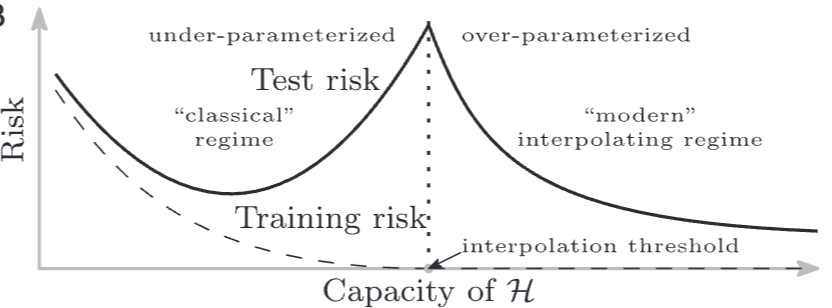
\includegraphics[width=\linewidth]{Deep-Learning-ETH-Summary-main/double_descent.png}

The NTK explains the interpolating regime, in particular why test accuracy decreases despite traing accuracy already being at 100\%. Assume a NN \(f : \mathbb{R}^d \times \mathbb{R}^n \to \mathbb R\).

\textbf{Neural Tangent Features:} \(\nabla_\theta f_\theta(x) \in \mathbb{R}^d\)\\
in analogy to generalized linear model \(f_\theta(x) = \theta^T \Phi(x)\)

\resizebox{\linewidth}{!}{\textbf{Neural Tangent Kernel (NTK):} $K_\theta(x,y) \!=\! \langle \nabla_\theta f_\theta(x), \nabla_\theta f_\theta(y) \rangle $}

\textbf{NTK Gram Matrix:} $K(\theta) \in \mathbb{R}^{s \times s}\quad K_{i,j}(\theta) = K_\theta(x_i, x_j)$

\textbf{Gradient Descent on sample $\{x_1, \ldots, x_s\}$ via NTK:}\\
Minimize \(\ell(\theta) = \frac{1}{2} \sum_{i=1}^s (f_\theta(x_i) - y_i)^2 \) via parameter gradient flow (ODE): \(\frac{d\theta}{dt} = - \nabla_\theta \ell(\theta) = \sum_{i=1}^s (y_i - f_\theta(x_i)) \nabla f_\theta(x_i)\).

\resizebox{\linewidth}{!}{\underline{Functional Gradient Flow:} $\frac{d f_\theta(x_j)}{dt} = \sum_{i=1}^s (y_i - f_\theta(x_i)) K_\theta(x_j, x_i)$}
which using the NTK Gram matrix gives $\frac{d \bf f}{dt} = K(\theta(t)) (\mathbf y - \mathbf f)$

\textbf{Linearize DNN around $\theta_0$ to get constant NTK $K_\theta = K$:}\\
$h(\vartheta)(x) = f_{\theta_0}(x) + \vartheta^T \nabla_\theta f_\theta(x) \vert_{\theta = \theta_0}  \quad \text{ where } \quad \vartheta = \theta - \theta_0$\\
Applying GD: $\vartheta \in \mathrm{span} \{\nabla_\theta f_\theta(x_1)|_{\theta=\theta_0}, \ldots, \nabla_\theta f_\theta(x_s)|_{\theta=\theta_0}\}$

\resizebox{\linewidth}{!}{Dual representation of minimizer: $\vartheta^* = \sum_{i=1}^s \alpha_i \nabla_\theta f_\theta(x_i)|_{\theta=\theta_0}$}

\resizebox{\linewidth}{!}{Loss function $\ell(\theta) = \frac{1}{2} \sum_{i=1}^s (\vartheta^T \nabla_\theta f_\theta(x_i)|_{\theta=\theta_0} - [y_i-f_{\theta_0}(x_i)])^2$}
Convex Kernel Regression: $\alpha^* = K^\dagger (\theta_0) (\bf y - \bf f_{\theta_0})$

Predict $f^*(x) = f_{\theta_0}(x) + K_{\theta_0}(x, (x_1, \ldots, x_s)) K^\dagger(\theta_0) (\bf y - \bf f_{\theta_0})$

\underline{DNN induces a random NTK whose Gradient Flow solu-}
\underline{tion approximates the optimal parameters to wide DNNs.}

\textbf{Nonlinear Deep Networks with constant NTK:}\\
Init $w_{ij}^l \sim \mathcal{N}(0,  \frac{\sigma_w^2}{m_l}), b_i^l \sim \mathcal{N}(0, \frac{\sigma_b^2}{m_l})$ at layer \(l\) with width \(m_l\).\\
In the infinite width limit \(m_l \to \infty\), $K_{\theta_0} \to K$ in probability, where $K$ depends on the model architecture and \(\sigma_w, \sigma_b\).

\underline{NTK Constancy}: In the $\infty$-width limit $\frac{d K_{\theta_t}}{dt} = 0$. We get a kernel machine 
$f^*(x) = f_{\theta_0}(x) + K(x, (x_1, \ldots, x_s)) K^\dagger (\bf y - \bf f_{\theta_0})$.
\underline{Emergence of constancy:} $\frac{||\nabla^2_\theta f_{\theta_0}(x)||_2}{||\nabla_\theta f_{\theta_0}(x)||_2^2 } \ll 1$ in the $\infty$-limit. Empirically, $||K(\theta_0) - K(\theta_t)||_F \in \mathcal{O}(\frac{1}{\sqrt{m}})$ over bounded \(\mathcal X\).